%%This is a very basic article template.
%%There is just one section and two subsections.
\documentclass[russian,utf8,pointsection]{eskdtext}
\usepackage{cmap}			% Поиск по русским словам в конечном pdf документе
\usepackage{eskdchngsheet}
\usepackage[T2A]{fontenc}
\usepackage{pscyr}			% Подключение "красивых" шрифтов киррилицы
\usepackage{amstext}
\usepackage{amsmath}


\usepackage{listings}		
\lstset{ %
	language=tcl,           % Язык программирования 	
	frame=single,           % Добавить рамку
	breaklines=true,        % Автоматический перенос строк
	breakatwhitespace=true, % Переносить строки по словам
	title=\lstname 
}

% работа с сылками
\usepackage{hyperref}
\usepackage[usenames,dvipsnames,svgnames,table,rgb]{xcolor}
\hypersetup{			
	unicode=true,           				% русские буквы в раздела PDF
	pdftitle={Заголовок},   				% Заголовок
	pdfauthor={Автор},      				% Автор
	pdfsubject={Тема},      				% Тема
	pdfcreator={Создатель}, 				% Создатель
	pdfproducer={Производитель}, 			% Производитель
	pdfkeywords={keyword1} {key2} {key3}, 	% Ключевые слова
	colorlinks=true,      					% false: ссылки в рамках; true: цветные ссылки
	linkcolor=NavyBlue,        				% внутренние ссылки
	citecolor=black,        				% на библиографию
	filecolor=black,        				% на файлы
	urlcolor=black          				% на URL
}

% Дает доступ к командам:
% \MakeTextUppercase{} - сделать все символы заглавными
\usepackage{textcase} 

%Изменение отображения Содержания
%\makeatletter
%\renewcommand{\l@section}{\@dottedtocline{1}{0em}{1.25em}}
%\renewcommand{\l@subsection}{\@dottedtocline{2}{1.25em}{1.75em}}
%\renewcommand{\l@subsubsection}{\@dottedtocline{3}{2.75em}{2.6em}}
%\makeatother

% Работа с таблицами
% p{} - top align, m{} - middle align, b{} - bottom align
\usepackage{ltablex} 										% longtable с функциональностю tabularx
\usepackage{multirow} 										% Слияние строк в таблице
\renewcommand{\tabularxcolumn}[1]{>{\arraybackslash}m{#1}}	% выравнивание в ячейке таблицы по середине по вертикали
\newcolumntype{M}[1]{>{\centering \arraybackslash}m{#1}} 	% колонка с заданной шириной и выравниванием по центру
\newcolumntype{Z}{>{\centering \arraybackslash} X} 			% колонка с выравниванием по центру


% Добавлено отображение Города на Титульном листе
\renewcommand{\ESKDtheTitleFieldX}{Екатеринбург \\ \ESKDtheYear}

% Уменьшен размер шрифта для заголовков секций
\ESKDsectStyle{section}{\large \bfseries \MakeTextUppercase}

% Выравнивание по центру.
% Предназначено для выравнивания надписей в шапке таблицы
\newcommand{\calign}[1]{\centering #1 \arraybackslash} 

%%% Работа с картинками
\usepackage{graphicx}  			% Для вставки рисунков
\graphicspath{{images/}}  % папки с картинками
\setlength\fboxsep{3pt} 		% Отступ рамки \fbox{} от рисунка
\setlength\fboxrule{1pt} 		% Толщина линий рамки \fbox{}
\usepackage{wrapfig} 			% Обтекание рисунков и таблиц текстом
\usepackage{float}

%%% Информация
\newcommand{\info}[1]{ %
\begin{flushleft}%
	\begin{tabular*}{\linewidth}{m{0.05\linewidth}m{0.9\linewidth}}%
		
\includegraphics[width=\linewidth]{info.jpg} & \textcolor{ForestGreen}{\textit{#1}}
	\end{tabular*}	
\end{flushleft}	
}

%%% Информация
\newcommand{\warning}[1]{ %
\begin{flushleft}%
	\begin{tabular*}{\linewidth}{m{0.05\linewidth}m{0.9\linewidth}}%
		
\includegraphics[width=\linewidth]{warning.jpg} & \textcolor{Red}{\textit{#1}}
	\end{tabular*}	
\end{flushleft}	
}

%%% Переопределение отображения счетчиков enumerate на отображение цифрами
\renewcommand{\theenumi}{\arabic{enumi}}
\renewcommand{\labelenumi}{\theenumi)}

\usepackage[backend=biber,bibencoding=utf8,sorting=ynt,maxcitenames=2,style=authoryear]{biblatex}
% \addbibresource{bib_orcad.bib}


% Заполнение граф Титульного листа и основной надписи
\ESKDcompany{ООО <<Прософт-Системы>>}
%\ESKDclassCode{} 
\ESKDtitle{Android Manual}
\ESKDdocName{Отдел Энергосвязи}
%\ESKDsignature{Заметки OrCAD 16.6}
\ESKDgroup{\normalsize ООО <<Прософт-Системы>>}

% основная надпись
\ESKDauthor{\ESKDfontII Щеблыкин М.В.}
%\ESKDchecker{\ESKDfontII Макаров Е.Г.}
%\ESKDnormContr{\ESKDfontII Бунина О.Ю.}
%\ESKDapprovedBy{\ESKDfontII Чирков А.Г.} 
\ESKDdate{2014/08/14}
%\ESKDcolumnI{АВАНТ К400 \\ \vspace{0.5cm} \ESKDfontIII{Инструкция по использованию протокола MODBUS}}

% переназначение в itemize символа первого уровня на жирную точку
\renewcommand\labelitemi{$\bullet$}

\begin{document}

\tableofcontents

\newpage
\section{Основные компоненты приложения. Жизненный цикл приложения}

Приложение само не решает когда завершиться, это делает ОС в тот момент, когда ей понадобятся ресурсы.

Приоритеты процессов:
\begin{itemize} 
	\item процесс переднего плана (который содержит Activity с которыми взаимодействует пользователь в данный момент или обрабатывается \\ BroadcastReceiver, или процессы содержащие foreground методы);
	\item видимый процесс (с которыми пользователь в данный момент не взаимодействует, но их UI виден пользователю);
	\item сервисный процесс (в котором запущен хотя бы один сервис);
	\item процесс заднего плана (которые содержат Activity не видимые пользователю в данный момент);
	\item пустой процесс (которые не содержат ни одного компонента, например, данные оставшиеся от убитой Activity).
\end{itemize}

% subsections
	%----
\subsection{Activity}
\textbf{Activity} --- одно окно приложения.

\begin{itemize}
	\item может занимать весь экран или его часть;
	\item может быть запущена из других компонент приложения или из другого приложения;
	\item может возвращать результат.
\end{itemize}

\begin{figure}[H]
    \centering
    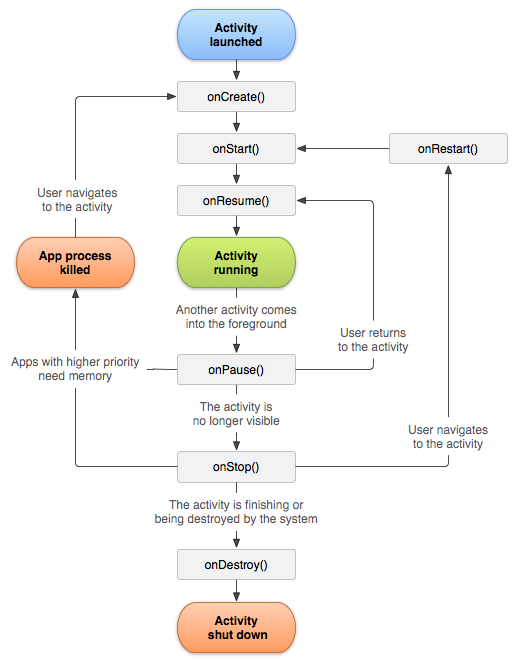
\includegraphics[width=0.5\textwidth]{activity_lifecycle}
    \caption{Жизненный цикл Activity}
    \label{fig:activity_lifecycle}
\end{figure}

На разных этапах существования Activity андроид вызывает различные методы, основные представлены на рисунке \ref{fig:activity_lifecycle}.

\begin{itemize}
	\item \textit{onCreate()} --- вызывается первым. В нем как правило создаются UI контролы.
	\item \textit{onStart()} --- вызывается в момент появления Activity на экране.
	\item \textit{onResume()} --- вызывается когда пользователь начинает взаимодействовать с Activity.
	\item \textit{onPause()} --- вызывается когда пользователь заканчивает работать с Activity. Если приложение осталось на экране и пользователь в дальнейшем возвращается обратно, идет вызов \textit{onResume()}.
	\item \textit{onStop()} --- вызывается когда Activity полностью уходит с экрана и перестает быть видимым.
	\item \textit{onRestart()} --- вызывается при возврате в Activity и далее \textit{onStart()}.
	\item \textit{onDestroy()} --- вызывается при сммене конфигурации или если пользователь закрыл Activity. Activity уничтожается.
\end{itemize}

Приложение может быть уничтожено после методов \textit{onPause()}, \textit{onStop()}. В этом случае следующие методы вызваны не будут, например \textit{onDestroy()}. За освобождение ресурсов при этом отвечает уже ОС.

\begin{figure}[H]
    \centering
    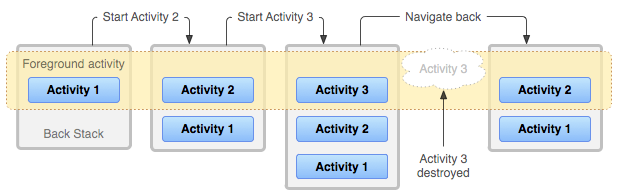
\includegraphics[width=0.8\textwidth]{diagram_backstack}
    \caption{Activity back stack}
    \label{fig:diagram_backstack}
\end{figure}

Как правило в приложении существует не одно Activity, а несколько. Когда пользователь вызывает из одной Activity другую, оно кладется сверху, а первая Activity уходит вниз (см. рисунок ). Таким образом образуется некий стек Activity. Когда пользователь нажимает кнопку \textit{back}, с этого стека верхняя Activity сносится, уничтожается и наверх поднимается та, что была под ней.

На рисунке \ref{fig:diagram_backstack} изображено поведение \textit{back stack} по умолчанию, которое можно изменять.

Для изменения поведения \textit{back stack} в Activity существует параметр \textit{Launch Modes}.
\begin{itemize}
	\item \textit{standart (default mode)} --- при каждом запуске Activity создается новый экземпляр Activiy и помещается на вершину \textit{back stack};
	\item \textit{singleTop} --- если в момент запуска экземпляр Activity уже находится на вершине стека, то новый экземпляр не создается, вместо этого вызывается метод \textit{onNewIntent()} у существующего экземпляра;
	\item \textit{singleTask} --- Activity запускается в отдельном \textit{Task}. Если экземпляр Activity уже существует, то у него вызывается метод \textit{onNewIntent()}, а все Activity лежащие в \textit{back stack} поверх этого экземпляра - уничтожаются.
	\item \textit{singleInstance} то же, что и \textit{singleTask}, но Activity является в своем таске единственной.
\end{itemize}


%----
\subsubsection{Пересоздание Activity}
	Android пересоздает Activity:
	\begin{itemize}
		\item при изменении конфигурации устройства, например когда изменяется ориентация экрана, пользователь меняет язык системы в настройках Android и т.п.;
		\item при возврате пользователя к процессу, который был убит Android для освобождения ресурсов.
	\end{itemize}
	
	
%----	
\subsubsection{Сохранение состояния при пересоздании Activity}

	\begin{figure}[H]
	    \centering
	    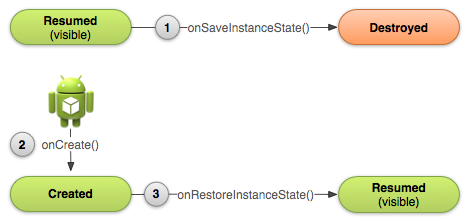
\includegraphics[width=0.8\textwidth]{basic_lifecycle_savestate}
	    \caption{Сохранение состояния при пересоздании Activity}
	    \label{fig:basic_lifecycle_savestate}
	\end{figure}
	
	\lstset{
	    language=java,
	    caption=Пример сохранения состояния при пересоздании Activity,
	    label=code:basicLifecycleSavestate_java,
	    keywordstyle=\color{blue}\bf,
	    commentstyle=\color{OliveGreen},
	    stringstyle=\color{red},
	    basicstyle=\scriptsize   
	}
	\lstinputlisting{files/basicLifecycleSavestate.java}
	
Если на Activity есть, например, EditText элемент в который пользователь может вбить свои строки, то нет необходимости специально сохранять этот текст, а достаточно вызвать суперметод в \textit{onSaveInstanceState}, либо не перекрывать его вообще. Отключить сохранение можно в свойствах элемента EditText.

Но таким образом сохранаются не все параметры элементов. Например, свойство \textit{visibility} не сохраняется и его можно сохранить отдельно (см. пример кода \ref{code:basicLifecycleSavestate_java}).

Не все объекты можно и нужно сохранять в \textit{Bundle}. Например, большие объемы данных будут сохраняться очень долго. 


%----	
\subsubsection{Сохранение объекта при пересоздании Activity}

\begin{itemize}
	\item методы \textit{onRetainNonConfigurationInstance / \newline getLastNonConfigurationInstance} --- \textbf{не рекомендуется};
	\item \textit{Static Field/Singleton/Application object}. \newline \textit{Singleton} --- существует один для всех экземпляров Activity, что может привести к проблемам, также не уничтожается вместе с Activity;
	\item \textit{Service} --- принципиально не отличается от \textit{Singleton}, но имеет дополнительные проблемы из-за асинхронности подключения к Activity;
	\item \textit{Retain Instance Fragment}.
\end{itemize}
	%----
\subsection{Service}
\textbf{Service} --- компонент для выполнения длительных фоновых задач.

\begin{itemize}
	\item не содержит графического интерфейса;
	\item может выполняться в том же процессе, что и само приложение, либо в отдельном;
	\item повышает значимость процесса с точки зрения Android.
\end{itemize}

Может быть использован, например, для проигрывания музыки в фоновом режиме.
	%----
\subsection{BroadcastReceiver}
\textbf{BroadcastReceiver} --- приемник широковещательных сообщений.

\begin{itemize}
	\item получает сообщения от Android или других приложений;
	\item Примеры широковещательных сообщений:
	\begin{itemize}
		\item BOOT
		\item SCREEN\_OFF/ON
		\item CONNECTIVITY\_ACTION
	\end{itemize}
	\item должен обрабатывать сообщения быстро, длительные задачи можно делегировать сервису.
\end{itemize}

При слишком долгом выполнении, например, порядка 10 секунд, Android может убить этот процесс. 
	%----
\subsection{Content Provider}
\textbf{Content Provider} --- компонент для доступа к хранилищу данных.

\begin{itemize}
	\item используется для доступа к данным, хранимым Android, или другими приложениями;
	\item приложение может давать доступ к своим данным для других приложений, реализуя Content Provider;
	\item предоставляет данные в виде таблиц, реализцет методы query, insert, update, delete.
\end{itemize}
	%----
\subsection{Intent}
\textbf{Intent} --- сущность для описания операции, которую требуется выполнить.

Используется для:
\begin{itemize}
	\item запуска Activity;
	\item запуска сервиса;
	\item отправки широковещательных сообщений;
	\item выполнения стандартных, преопределенных операций.
\end{itemize}
	%----
\subsection{Application}
\textbf{Application} --- существует в любом Android приложении. 
Создается вместе с процессом и первым вызывается метод \textit{onCreate()}, в котором удобно инициализировать собственные компоненты или сторонние библиотеки, т.к. вызывается до старта любых Activity, сервисов и т.д.

Метод \textit{onConfigurationChanged()} вызывается когда меняется конфигурация ОС. Например, когда меняется ориентация экрана, подключается клавиатура и т.д.
	%----
\subsection{Task}
\textbf{Task} --- множество Activity.  

Внутри лежит \textit{back\_stack}. Может уйти в \textit{background} и быть возвращенным в \textit{foreground}. 
	%----
\subsection{AndroidManifest.xml}

В файле \textit{AndroidManifest.xml} описываются все компоненты Android приложения.
 
\lstset{
    language=xml,
    caption=Пример объявления компонента Activity,
    label=code:activity_xml,
    keywordstyle=\color{blue}\bf,
    commentstyle=\color{OliveGreen},
    stringstyle=\color{red},
    basicstyle=\scriptsize    
}
\lstinputlisting{files/activity.xml}
\begin{ESKDexplanation}
\item[где ] \textit{activity name} --- имя класса который реализует Activity в java;
\item \textit{activity lable} --- заголовок Activity;
\item \textit{activity windowSoftInputMode} --- указано что должна быть скрыта программная клавиатура;
\item \textit{activity launchMode} --- задано значение \textit{singleTask};
\item \textit{intent-filter action name} --- показывает что это главная Activity приложения, та с которой начнется запуск приложения;
\item \textit{intent-filter category name} --- показывает что Activity будет присутствовать в Laucnher-е Android, т.е. в списке всех приложений. 
\end{ESKDexplanation}

\subsubsection{Параметр configChanges}
	В этом параметре можно указать при каких изменениях мы не хотим чтобы Android пересоздавал Activity. Вместо этого будет вызван метод \textit{onConfigurationChanged()}, в котором мы обработаем смену конфигурации самостоятельно.
	 
	 
В пример ниже, при повороте экрана просто показывается его текущее состояние.
	\begin{center}
	android:configChanges=``orientation|ScreenSize''
	\end{center}
	
	\lstset{
	    language=java,
	    caption=Пример обработчика изменения конфигурации,
	    label=code:onConfigurationChanged_java,
	    keywordstyle=\color{blue}\bf,
	    commentstyle=\color{OliveGreen},
	    stringstyle=\color{red},
	    basicstyle=\scriptsize   
	}
	
	\lstinputlisting{files/onConfigurationChanged.java}
	
\warning{Использование параметра \textit{configChanges} не избавляет от необходимости корректно обрабатывать пересоздание Activity. \newline Оно оправдано только в редких, исключительных случаях!}
	
\end{document}
